\RequirePackage{amsthm} %https://tex.stackexchange.com/questions/687324/unknown-theoremstyle-warning-with-springer-nature-template
\documentclass[sn-mathphys-num,iicol]{sn-jnl}

%\usepackage{sn-jnl.sty}
\usepackage{graphicx}%
\usepackage{multirow}%
\usepackage{amsmath,amssymb,amsfonts}%
\usepackage{amsthm}%
\usepackage{physics}
\usepackage{siunitx}
\usepackage{mathrsfs}%
\usepackage[title]{appendix}%
\usepackage{xcolor}%
\usepackage{textcomp}%
\usepackage{manyfoot}%
\usepackage{booktabs}%
\usepackage{algorithm}%
\usepackage{algorithmicx}%
\usepackage{algpseudocode}%
\usepackage{listings}%
\usepackage{newtxmath}%
\usepackage[tiny]{titlesec}%

\theoremstyle{thmstyleone}
\newtheorem{theorem}{Theorem}
\newtheorem{proposition}[theorem]{Proposition}

\theoremstyle{thmstyletwo}
\newtheorem{remark}{Remark}

\theoremstyle{thmstylethree}
\newtheorem{definition}{Definition}

\raggedbottom

\newcommand{\td}{\text{d}}

\titleformat{\subsection}{}{\thesubsection}{1em}{\itshape}

\begin{document}
        
\title[Title]{Das Magnetische Moment des Protons}
\author*[1]{\fnm{Jonas} \sur{Wortmann}}\email{s02jwort@uni-bonn.de}
\affil*[1]{Rheinische Friedrich--Wilhelms--Universität, Bonn}

\abstract{Es wird das magnetische Moment des Protons in Bezug auf seine historische Bedeutung als erstes Indiz für die Substruktur des Protons erläutert.
Dafür wird das der experimentelle aus 1933 Aufbau von \textsc{Frisch} und \textsc{Stern} zur Bestimmung des Protonenmoments erklärt, die Auswertung dargestellt und das Ergebnis in Hinblick auf die damalige Erwartung diskutiert.
Zu Beginn wird kurz die Entdeckung des Protons durch \textsc{Rutherford} und das magnetische Moment und Magneton dargestellt.
Im Anschluss wird ein kurzer Ausblick in aktuelle Forschungsthemen besprochen.}

\maketitle

\section{Einleitung}
Das Protonenmoment ist eine sehr wichtige physikalische Größe, nicht nur in historischer Betrachtung, sondern auch vor aktuellem Forschungshintergrund.

Historisch führte das Protonenmoment zu Überlegungen über den Aufbau der Protonen.
Durch Messung des magnetischen Moments konnte im Vergleich mit den Erwartungen, die aus den damals gängigen Theorien angestellt werden konnten, erkannt werden, dass die Theorie des Protons den experimentellen Ergebnissen nicht genügt.

In aktueller Forschung findet sich das Protonenmoment vor Allem im Vergleich mit dem Antiprotonenmoment, um Aussagen über die CPT--Symmetrie und Materie--Antimaterie Asymmetrie zu treffen.
Ein großer Anwendungsbereich ist die Magnetresonanztomographie in der Medizin, die es ermöglicht, ohne schädliche Strahlung, Bilder von Gewebe zu erzeugen.

\section{Die Entdeckung des Protons}
Die Entdeckung des Protons wird im allgemeinen \textsc{Rutherford} um 1920 zugeschrieben.

In einem Experiment um 1933 haben \textsc{Rutherford} und \textsc{Mardsen} ein Gasgemisch (Luft) mit $\alpha $--Teilchen beschossen, um den inneren Aufbau der Atome zu erforschen.

Die $\alpha $--Teilchen stammen von einer radioaktiven Probe, dessen Teilchenstrahl auf Luft gerichtet ist.
In Verlängerung der Probe und Luft ist ein Zinksulfidschirm angebracht.
Die Entfernung des Schirms von dem Gas ist wesentlich größer als die Reichweite der $\alpha $--Strahlung, um zu vermeiden, diese auf dem Schirm detektiert werden.

Das Ergebnis des Experiments liefert, dass die $\alpha $--Teilchen mit der Luft stoßen und dabei Wasserstoffkerne aus dem Gas lösen, welche als Aufblitzen auf dem Schirm beobachtet werden können.

Eine wichtige Schlussfolgerung hat \textsc{Rutherford} aufgestellt, als er das Experiment mit Stickstoff anstatt Luft wiederholt hat.
Auch bei Stickstoff konnte das selbe Aufblitzen wie bei Luft beobachtet werden.
Daraus schloss er, dass Stickstoff aus Wasserstoffkernen bestehen muss.

Die Entdeckung des Protons wird einer Aussage um 1920 von \textsc{Rutherford} zugeschrieben, bei der er seine Beobachtungen aus dem Experiment 1933 verallgemeinerte.
Er behauptete, dass jedes Atom aus Wasserstoffkernen bestehen musste.
Zur Unterscheidung von ionisiertem Wasserstoff, nannte er diese Bestandteile Protonen.\cite{Rutherford_proton_discovery}\cite{Rutherford1919}

\section{Das magnetische Moment und das Magneton}
Die klassische Betrachtung des magnetischen Moments des Protons liefert die Stärke und Richtung eines magnetischen Dipols $\boldsymbol{m}=\tfrac{1}{2}\int\td ^3r\left[\boldsymbol{r} \times \boldsymbol{j} \left(\boldsymbol{r} \right)\right]$.
Betrachtet man einen Strom der um eine Fläche kreist, so ergibt sich der Ausdruch $\boldsymbol{m} =I\cdot \boldsymbol{A} $.
Betrachtet man den Kreisstrom erzeugt von einem geladenen Teilchen auf einer Kreisbahn, so ergibt sich mit $I=q/T$, mit $T$ der Periodendauer und $q$ der Ladung, und der Kreisfläche $|\boldsymbol{A} |=\pi r^2$ ein Moment von $|\boldsymbol{m} |=\tfrac{q}{T}\pi r^2$.
Der Bahndrehimpuls eines Teilchens auf einer Kreisbahn ist beschrieben durch $|\boldsymbol{l} |=\tfrac{2\pi }{T}mr^2$.
Bahndrehimpuls und magnetisches Moment lassen sich also miteinander verbinden zu $|\boldsymbol{\mu } |:=|\boldsymbol{m} |=\gamma |\boldsymbol{l} |=\tfrac{q}{2m}|\boldsymbol{l} |$.
Diese Größe wird auch als Magneton bezeichnet.

Die quantenmechanische Betrachtung des Magnetons liefert dann diskrete Werte, die proportional zu den Eigenwerten von $\hat{l}_z$ sind.
Wichtig für die folgende Diskussion sind das \textsc{Bohr}'sche Magneton für Elektronen mit der Drehimpulsquantenzahl $\ell=1$: $\mu _B=\tfrac{e\hbar }{2m_e}$; und das Kernmagneton, eine gängige Einheit in der Teilchenphysik, für Teilchen mit Spin $\tfrac{1}{2}$, $\ell=1$ und der Protonmasse: $\mu _N=\tfrac{e\hbar }{2m_p}$.

\section{Das Experiment von Otto Robert \textsc{Frisch} und Otto \textsc{Stern}}
\subsection{Motivation}
Die Motivation hinter diesem Experiment ist die Untersuchung des Wasserstoffs mit dem Ziel einer Bestimmung des Protonenmoments.
Darüber hinaus soll auch eine allgemeine Apparatur zur Messung magnetischer Momente in der Größenordnung eines Kernmagnetons $\mu _N$ errichtet werden.
Die kürzliche Entdeckung des Ortho-- und Para--Wasserstoffmoleküls sind hierfür nützlich und wollen auch untersucht werden.

\subsection{Experimenteller Aufbau}
\begin{figure}[h]
        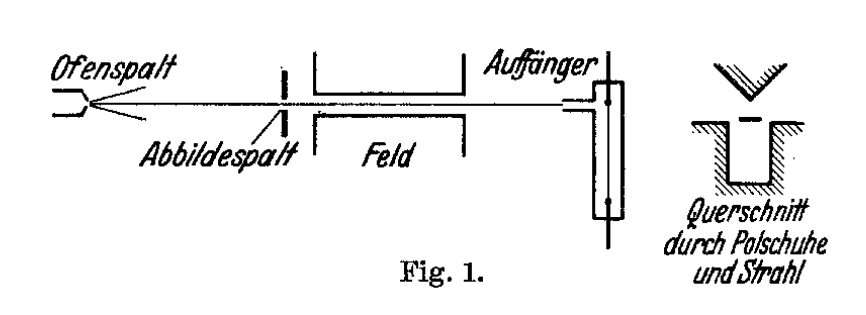
\includegraphics[width=.5\textwidth]{../vortrag/prosi_versuchsaufbau_mag_moment.png}
        \caption{Experimenteller Aufbau (schematisch); Gesamtlänge $\SI{30}{cm}$.\cite{FrischStern1933}}\label{fig:experimenteller_aufbau_frisch_stern}
\end{figure}
\noindent Der schematische experimentelle Aufbau ist in (\ref{fig:experimenteller_aufbau_frisch_stern}) gezeigt.
Aus dem Ofen tritt ein Molekülstrahl ($\text{H}_2$) aus, der mit Hilfe eines Abbildespaltes kollimiert wird und dann in ein inhomogenes Magnetfeld eintritt.
In diesem Feld wird der Strahl abgelenkt und die Intensität kann mit Hilfe des Auffängers (Manometer) gemessen werden.
Das Feld entsteht durch Polschuhe, deren Querschnitt abgebildet ist.
Auf die exakte Anordnung und weitere technische Details wird hier nicht eingegangen.
Diese sind ausführlich in der Originalarbeit\cite{FrischStern1933} erklärt.

Es werden kurz die Anforderungen und Schwierigkeiten beschrieben.
Der Strahl muss aufgrund der kleinen magnetischen Momente sehr lang und schmal sein, damit die Abweichungen durch das Feld entsprechend groß sind und genaue Messungen angestellt werden können.
Der kleinste im Experiment verwendete Strahl hat einen Durchmesser von circa $\SI{0.03}{mm}$.
Wichtig sind auch große Inhomogenitäten des Feldes.
Diese liegen im Bereich von circa $\SI{22}{T/cm}$.
Für einen Strahl mit einem magnetischen Moment von einem Kernmagneton ist dann eine Abweichung von $s=\SI{0.0044}{mm}$ zu erwarten.

Besondere Schwierigkeiten ergeben sich aus der Natur des Molekülstrahls ($\text{H}_2$).
Dieser Strahl ist \textsc{Maxwell}--verteilt, was dazu führt, dass die Moleküle unterschiedliche Geschwindigkeiten haben und dadurch unterschiedlich starke Ablenkungen erfahren.
Aus diesem Grund kann die Ablenkung -- alleine verursacht durch das magnetische Moment -- nicht abgelesen werden, sondern muss es aus der Intensitätsverteilung berechnet werden.
Solch kleine Intensitäten können mit Hilfe von sehr empfindlichen Manometern gemessen werden.
Technische Details sind in der Originalarbeit\cite{FrischStern1933} zu finden.

\subsection{Erwartung}
Die Erwartung des Experiments gibt für das Protonenmoment einen Wert von exakt $\mu _p=1\cdot \mu _N=1\cdot \tfrac{e\hbar }{2m_p}$ an.
Diese Erwartung beruht auf der Annahme, dass das Proton ein elementares \textsc{Dirac}--Teilchen ist; also punktförmig und ohne innere Struktur.
Diese Annahme liegt in anbetracht des wissenschaftlichen Standes sehr nahe, da unter anderem das Elektron passend durch die \textsc{Dirac}'sche--Theorie beschrieben ist.

Der Wert des Protonenmoments sollte sich also, nur aufgrund des Massenunterschieds, um einen Faktor von circa 1840 von dem des Elektrons unterscheiden.\cite{FrischStern1933}

\subsection{Durchführung \& Auswertung}
Das Gesamtmoment des $\text{H}_2$ ist eine Zusammensetzung aus dem Rotationsmoment und dem Kernmoment.
Das Kernmoment ist nicht exakt das Protonenmoment, da es sich hier um das $\text{H}_2$--Molekül handelt; das Protonenmoment kann aber aus dem Kernmoment berechnet werden.

Die Beobachtung und Auswertung werden an Ortho-- und Parawasserstoffmolekülen durchgeführt, da ihre magnetischen Eigenschaften sehr nützlich sind.

Das $\text{H}_2$--Molekül hat zwei verschiedene, aufgrund des \textsc{Pauli}--Prinzips, mögliche Spinanordnungen.
In Ortho--$\text{H}_2$ ist die Ausrichtung $\ket{\uparrow\uparrow}$ zu finden; in Para--$\text{H}_2$ $\ket{\uparrow\downarrow}$.
Die Auswirkung davon ist, dass Ortho--$\text{H}_2$ ein Kernmoment von ungleich null und Para--$\text{H}_2$ ein Kernmoment von gleich null hat.
Für beide Arten des Moleküls erwartet man also verschiedene Aufspaltungsbilder.
In (\ref{fig:ortho_aufspaltung}) ist dies beispielhaft für Ortho--$\text{H}_2$ gezeigt. 
\begin{figure}[h]
        \centering
        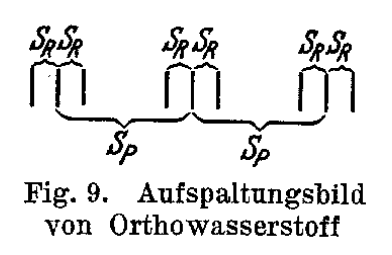
\includegraphics[width=.3\textwidth]{../vortrag/prosi_aufspaltungsbild_orthowasserstoff.png}
        \caption{Das Aufspaltungsbild von Ortho--$\text{H}_2$.\cite{FrischStern1933}} \label{fig:ortho_aufspaltung}
\end{figure}
Dabei beschreibt $S_R$ die Aufspaltung aufgrund des Rotationsmoments und $S_p$ die Aufspaltung aufgrund des Kernmoments.

Ziel dieser Auswertung ist die Bestimmung des Kernmoments, um Rückschlüsse auf das Protonenmoment zu ziehen.
Dafür muss zuerst das Rotationsmoment von $\text{H}_2$ bestimmt werden, um dieses im Anschluss von dem Gesamtmoment zu subtrahieren.
Die Berechnung folgt aus der Intensitätsverteilung von Para--$\text{H}_2$ (zu sehen für gewöhnliches $\text{H}_2$ in (\ref{fig:graph})), da eine Bestimmung durch Ablesen der Ablenkung des Strahls aufgrund der Messgenauigkeit nicht möglich ist.
Es wird Para--$\text{H}_2$ verwendet, da dies ein Kernmoment von null hat und das Gesamtmoment nur aus dem Rotationsmoment besteht.
\begin{figure}[h]
        \centering
        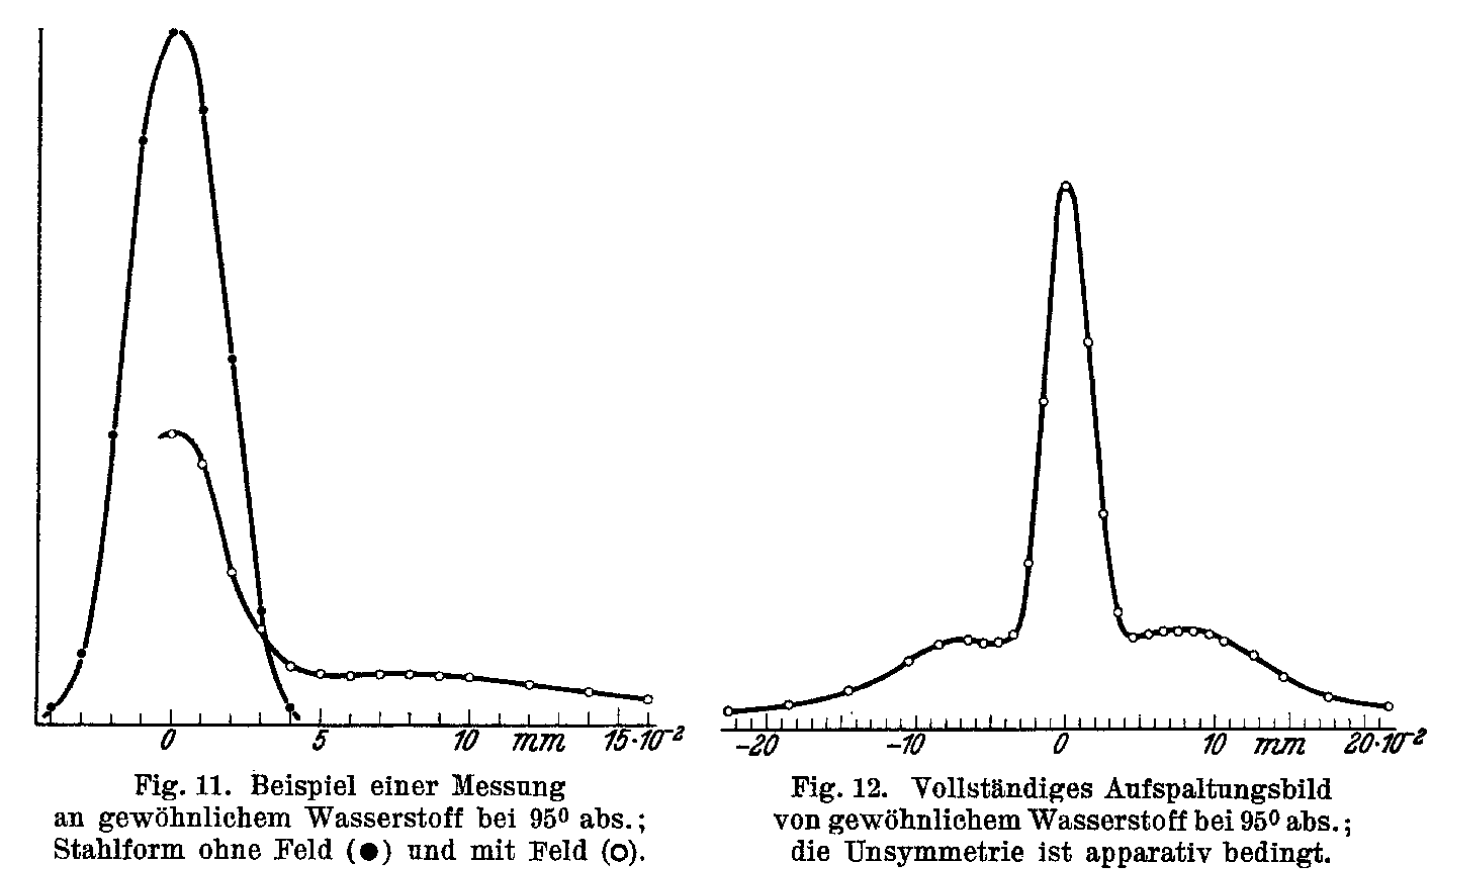
\includegraphics[width=.5\textwidth]{../vortrag/prosi_frisch_stern_auswertung_graph.png}
        \caption{Intensitätsverteilung des Molekülstrahls. Rechts ist eine Vergrößerung.\cite{FrischStern1933}} \label{fig:graph}
\end{figure}
Para--$\text{H}_2$ ist \textsc{Boltzmann}--verteilt, was bedeutet, dass $73\%$ der Moleküle die Rotationsquantenzahl $n=0$ und $27\%$ $n=2$ haben.
Für den Anteil mit $n=0$ ergibt sich keine Ablenkung, was dem Peak der Intensitätsverteilung um die Ablenkung von $\SI{0}{mm}$ entspricht.
Für den Anteil mit $n=2$ ergibt sich eine Aufspaltung aufgrund der Aufhebung der Entartung.
Man erhält dann jeweils Anteile der Intensitäten von $\tfrac{1}{5}$ für $m_n  \in \left\{-2,-1,0,+1,+2\right\}$ die je einen abiträres Rotationsmoment (--quant) von $m_n\cdot \mu _R$ besitzen.
Es ergibt sich also ein analoges Bild zu (\ref{fig:ortho_aufspaltung}) nur mit 5 anstatt 9 Intensitätsmaxima.

Dieses Rotationsmoment $\mu _R$ wird dann über folgende Methode bestimmt.
Man berechnet eine erwartete Intensität für ein bestimmtes $\mu _R$ und vergleicht diese dann mit der tatsächlich gemessenen Intensität.
Stimmen diese Intensitäten nicht überein, so wird $\mu _R$ weiter variiert.
Für ein bestimmtes $\mu _R$, was genau dem Rotationsmoment des Molekülstrahls entspricht, sind die Intensitäten gleich.

Das Rotationsmoment von Para--$\text{H}_2$ ergibt sich dann zu $\mu _R\lesssim \mu _N$.
Dieses Rotationsmoment ist auch der Wert für gewöhnliches $\text{H}_2$.
Misst man also das Gesamtmoment über die selbe Methode so kann das Kernmoment von $\text{H}_2$ berechnet werden.\cite{FrischStern1933}

\subsection{Ergebnis}
Die im vorigen Abschnitt diskutierte Auswertung gibt für das magnetische Moment des Protons einen Wert von $3\mu _N\leq \mu _p\leq 5\mu _N$.
Dieses Ergebnis ist nicht mit der Erwartung von $\mu p=\mu _N$ vereinbar.\cite{FrischStern1933}

Aus moderner Forschungsperspektive ist dieses Ergebnis allerdings sehr gut zu erklären.
Das Proton ist kein elementares Punktteilchen, sondern ein aus Quarks zusammengesetztes Teilchen; $\left(u,u,d\right)$.
Das Protonenmoment berechnet sich also aus dem Moment der Quarks mit $\mu _p=\tfrac{3}{4}\mu _u-\tfrac{1}{3}\mu _d\approx 2.792\mu _N$\cite{CODATA_proton_magneton}.

Obwohl dieses Ergebnis in der Originalarbeit noch nicht gedeutet werden konnte, ist es dennoch ein wichtiges Ereignis, bei dem die Struktur des Protons erstmals in Frage gestellt wurde.

\section{Die Substruktur des Protons}
Eine genaue Betrachtung der Substruktur von Teilchen haben zum ersten Mal \textsc{Gell--Mann}\cite{Gellmann1964} und \textsc{Zweig}\cite{Zweig1964} 1964 unabhängig voneinander angestellt.

\textsc{Gell--Mann}\cite{Gellmann1964} stellt ein Modell dar, indem Teilchen aus anderen Teilchen, namentlich \textit{Quarks}, aufgebaut werden können.
Es ergibt sich, dass Baryonen aus einer ungeraden Anzahl an Quarks, also $\left(q,q,q\right)$, $\left(q,q,q,q,\overline{q}\right)$ etc.\ und Mesonen aus einer geraden Anzahl, also $\left(q,\overline{q}\right)$, $\left(q,q,\overline{q},\overline{q}\right)$ etc.\ aufgebaut werden können.
Weiter geht er darauf ein, dass mit diesem Modell der von ihm beschrieben \textit{Eightfold Way} zur Kategorisierung von Teilchen dargestellt werden kann.

Eine analoge, allerdings nicht auf dem \textit{Eightfold Way} beruhende Erklärung wird auch von \textsc{Zweig}\cite{Zweig1964} geliefert.
In seiner Ausarbeitung stellt er die Elementarteilchen als Aces vor.

Dieses Modell wurde kurz nach Veröffentlichung beider Arbeiten am SLAC (Stanford Linear Accelerator Center) Experiment bestätigt.\cite{Bloom1969}
Aus Elektron -- Proton Streuung wurde die Strukturfunktion gemessen, welche ergab, dass die Ladungsverteilung des Protons (an dem die Elektronen streuuen) punktförmig sein musste.
Dieses Ergebnis wurde in einer Ausarbeitung diskutiert und man hat diese punktförmige Ladungsverteilung mit den Quarks von \textsc{Gell--Mann} identifiziert.

\section{Aktuelle Forschung}
In der modernen Forschung findet das Protonenmoment eine große Bedeutung, vor Allem im Hinblick auf die CPT--Symmetrie und Materie--Antimaterie Asymmetrie.
Anwendung findet das Protonenmoment in der Medizin, im Hinblick auf die Magnetresonanzspektroskopie.
Es sollen kurz beide Punkte angerissen werden.

Am BASE im Cern\cite{BASE2017} wird mit Hilfe von zwei \textsc{Penning}--Fallen das magnetische Moment des Antiprotons gemessen und mit dem magnetischen Moment des Protons verglichen.
Dabei können die Zyklotronfrequenz und \textsc{Lamor}präzession jeweils separat gemessen werden, um eine möglichst hohe Auflösung zu erreichen.
Es wird nach Diskrepanzen gesucht, die zu möglichen Symmetriebrechungen führen könnten.

Das MRT beruht auf der Spin--Gitter und Spin--Spin Relaxation der Protonen in einem (organischen) Material.
Die Spins werden mit Hilfe eines homogenen Magnetfeldes ausgerichtet und dann durch Impulse (magnetische Wechselfelder) ausgelenkt.
Diese Auslenkung ruft zwei Effekte hervor:
Die Spin--Gitter Relaxation, bei der sich die Protonenspins langsam entlang der homogenen Magnetfeldlinien ausrichten und dabei eine Änderung der Magnetisierung in der zum Feld orthogonalen Ebene gemessen werden kann;
die Spin--Spin Relaxation, bei der sich die Magnetisierung innerhalb der orthogonalen Ebene aufgrund der unterschiedlichen Präzessionsgeschwindigkeiten der Protonenspins ausgleicht.
Bei beiden Relaxationsprozessen wird eine Magnetisierung gemessen, die mit Hilfe von Algorithmen als Bilder von Spindichten interpretiert werden kann.
Diese geben Aufschlüsse über die Struktur der (organischen) Materie.

\bibliography{refs}

\end{document}
